\documentclass{beamer}

\usepackage[utf8]{inputenc}
\usetheme{Warsaw}

\title{Embedded Systems - Bachelor Project}
\author{Moritz Herzog, Philipp Lersch}
\date{\today}

\usepackage{tikz}
\usetikzlibrary{shapes.geometric, arrows, chains, calc}

\tikzset{
    green/.style  = {draw, rectangle, minimum width=2cm, minimum height=1cm, text centered, text width=1.2cm, font=\footnotesize, draw=black, fill=green!30},
    blue/.style   = {draw, rectangle, minimum width=8cm+3\pgflinewidth, minimum height=1cm, text centered, text width=5.0cm, font=\footnotesize, draw=black, fill=blue!30},
    yellow/.style = {draw, rectangle, minimum width=8cm+3\pgflinewidth, minimum height=1cm, text centered, text width=5.0cm, font=\footnotesize, draw=black, fill=yellow!30},
}

\addtobeamertemplate{navigation symbols}{}{%
    \usebeamerfont{footline}%
    \usebeamercolor[fg]{footline}%
    \hspace{1em}%
    \insertframenumber/\inserttotalframenumber
}

\AtBeginSection[]
{
  \begin{frame}
    \frametitle{Table of Contents}
    \tableofcontents[currentsection]
  \end{frame}
}

\begin{document}
\maketitle


\section{OpenCL}
\begin{frame}
    \frametitle{OpenCL Structure}
    \begin{columns}
        \column{.6\textwidth}
        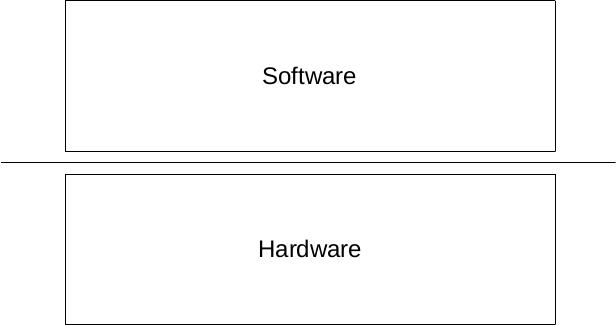
\includegraphics[width=\textwidth]{res/HardwareSoftwareLayer.jpg}
        \column{.4\textwidth}
        \begin{itemize}
            \item OpenCL draws clear line between hardware and software
        \end{itemize}
    \end{columns}
\end{frame}
\subsection{Hardware Model}
\begin{frame}
    OpenCL Propertys:
    \begin{itemize}
     \item Diffrent Models for CPU and GPU
    \end{itemize}
\end{frame}
\begin{frame}
    \frametitle{Hardware Model - Memory}
    \begin{itemize}
     \item Some Memeory Stuff
    \end{itemize}
\end{frame}
\begin{frame}
    \frametitle{Hardware Model - CPU}
    \begin{itemize}
     \item Some CPU Stuff
    \end{itemize}
\end{frame}
\begin{frame}
    \frametitle{Hardware Model - GPU}
    \begin{itemize}
     \item Some GPU Stuff
    \end{itemize}
\end{frame}
\subsection{Software Model}
\begin{frame}
    \frametitle{Software Model}
\end{frame}

\section{Kernels}
\begin{frame} %%Eine Folie
  \frametitle{List of Kernels} %%Folientitel
  Already there:
  \begin{itemize}
   \item Battery
   \item Speed
   \item Acceleration
   \begin{itemize}
    \item X-Achsis
    \item Y-Achsis
    \item Tangential
   \end{itemize}
   \item Tempreture
  \end{itemize}

  %\begin{Definition} %%Definition
  %  Eine Definition
  %\end{Definition}
\end{frame}
\begin{frame}
    \frametitle{List of Kernels}
    Added Kernels:
    \begin{itemize}
     \item Tractioncontrol
     \item Accident Detection
     \item Anti-Lock Braking System
    \end{itemize}
\end{frame}
\subsection{Tractioncontrol}
\begin{frame}
    \frametitle{Accident Detection}
    By testing for accelerationspikes or accelerationvalues, we are able to detect accidents and unexpected movement.\\
    \begin{itemize}
     \item Check for values above or below given thresholds which should be unachieveable under normal circumstances.\\
     $\Rightarrow$ If found, we crashed.
     \pause
     \item In addition we can look for spikes in the last n-datapoints of the acceration and determine light crashes.\\
     $\Rightarrow$ If found, we crashed.
     \pause
    \end{itemize}
\end{frame}
\subsection{Anti Blocking System}
\begin{frame}
    \frametitle{Anti Blocking System}
    By comparing the fronts average and back wheels speeds we can determine if the rear wheels are turning to slow or are locking up. 
    \begin{itemize}
     \item Check if the rear wheels are spinning much slower (threshold is around 40\%) than the front wheels.\\
     $\Rightarrow$ If this is true for one or both wheels we are breaking to hard.\\
     $\Rightarrow$ Signal traction loss.
     \pause
     \item We could also try to regain traction by spinning the motor a little bit faster until we regain traction and slow down again.\\
     $\Rightarrow$ Hard to implement without proper or near realtime capeabliltys and no finer specified wheel control. Breaking has to be implemented by slowing down the build in motor. \\
     \pause
    \end{itemize}
\end{frame}
\subsection{Drive Slip Control}
\begin{frame}
    \frametitle{Drive Slip Control}
    By comparing the fronts average and back wheels speeds we can determine if the rear wheels are turning to fast. 
    \begin{itemize}
     \item Check if the rear wheels are spinning much faster (threshold is around 40\%) than the front wheels.\\
     $\Rightarrow$ If this is true for one or both wheels we are accelerating to hard.\\
     $\Rightarrow$ Signal traction loss.
     \pause
     \item We could also try to regain traction by spinning the motor a little bit slower until we regain traction and slow down again.\\
     $\Rightarrow$ Hard to implement without proper or near realtime capeablilties and no finer specifieable wheel control like a differential lock. Could be implemented by flattening the acceleration curve for the motor. \\
     \pause
    \end{itemize}
\end{frame}
\subsection{Tractioncontrol}
\begin{frame}
    \frametitle{Tractioncontrol}
    By comparing the fronts average and back wheels speeds we can determine if the rear wheels have lost to much traction.
    \begin{itemize}
     \item Check if the rear wheels are spinning outside of their thresholds.\\
     $\Rightarrow$ If one or both wheels are to slow we are breaking to hard.\\
     $\Rightarrow$ Signal traction loss.\\
     $\Rightarrow$ If one or both wheels are to fast we are accelerating to hard.\\
     $\Rightarrow$ Signal traction loss.
     \pause
     \item Without the needed capeablilties we are only cabealbe to signal the loss of traction.
     \pause
    \end{itemize}
\end{frame}
\subsection{Range}
\begin{frame}
    \frametitle{Range}
    Requirements:
    \begin{itemize}
        \item Knowlegde of the maximum Battery Charge in Wh
        \item Minimum charge voltage
        \item Engine propertys (load to watt usage)
    \end{itemize}
\end{frame}
\begin{frame}
    \frametitle{Range}
    Algorithm
    \begin{enumerate}
     \item Get current battery voltage
     \item Calculate current charge in Wh
     \item Calculate on engine load, engine proppertys and current speed the current consumed wattage
     \item Calculate the remaining Range with these Formulars.
     \begin{itemize}
        \item $remainingTime=\frac{Charge}{Current Wattage}\cdot3600$
        \item $remainingRange=speed\cdot remainingTime$
     \end{itemize}
    \end{enumerate}
\end{frame}
\subsection{Turningradius}

\begin{frame}
    \frametitle{Turningradius}
    Requirements:
    \begin{itemize}
     \item wheel Velocity of every wheel sepread ($\Sigma_{RR}$, $\Sigma_{RL}$, $\Sigma_{FR}$, $\Sigma_{FL}$)
     \item Knowlegde of the width of the axle (Distance of the two wheels on one axle) ($D$)
    \end{itemize}
    Algorithm:
    \begin{enumerate}
     \item Calculate the folloring Formular
     \begin{itemize}
        \item $r=\frac{D}{2}*\frac{\Sigma_{RR}+\Sigma_{RL}}{\Sigma_{RR}-\Sigma_{RL}}$
        \item Same can be done for the front axle to calculate slippige
     \end{itemize}
     \item if $r<0$ then $r=-r$
    \end{enumerate}
\end{frame}

\end{document}
